\section{6FLAS: Lightweight Security Mechanism}
\label{sec:method}

6FLAS addresses the LEO resource constraints by moving all per-flow security
context out of the satellite and into the packet. A domain key shared among
authorized nodes lets every on-board router verify each packet with a single
short keyed MAC, while an SRv6 Security SID encodes the per-hop path policy
and exploits the fixed LEO forwarding topology for constant-time access control.
The only mutable on-board state is a small per-direction replay window,
independent of the flow count.

\begin{figure}[t]
\centering
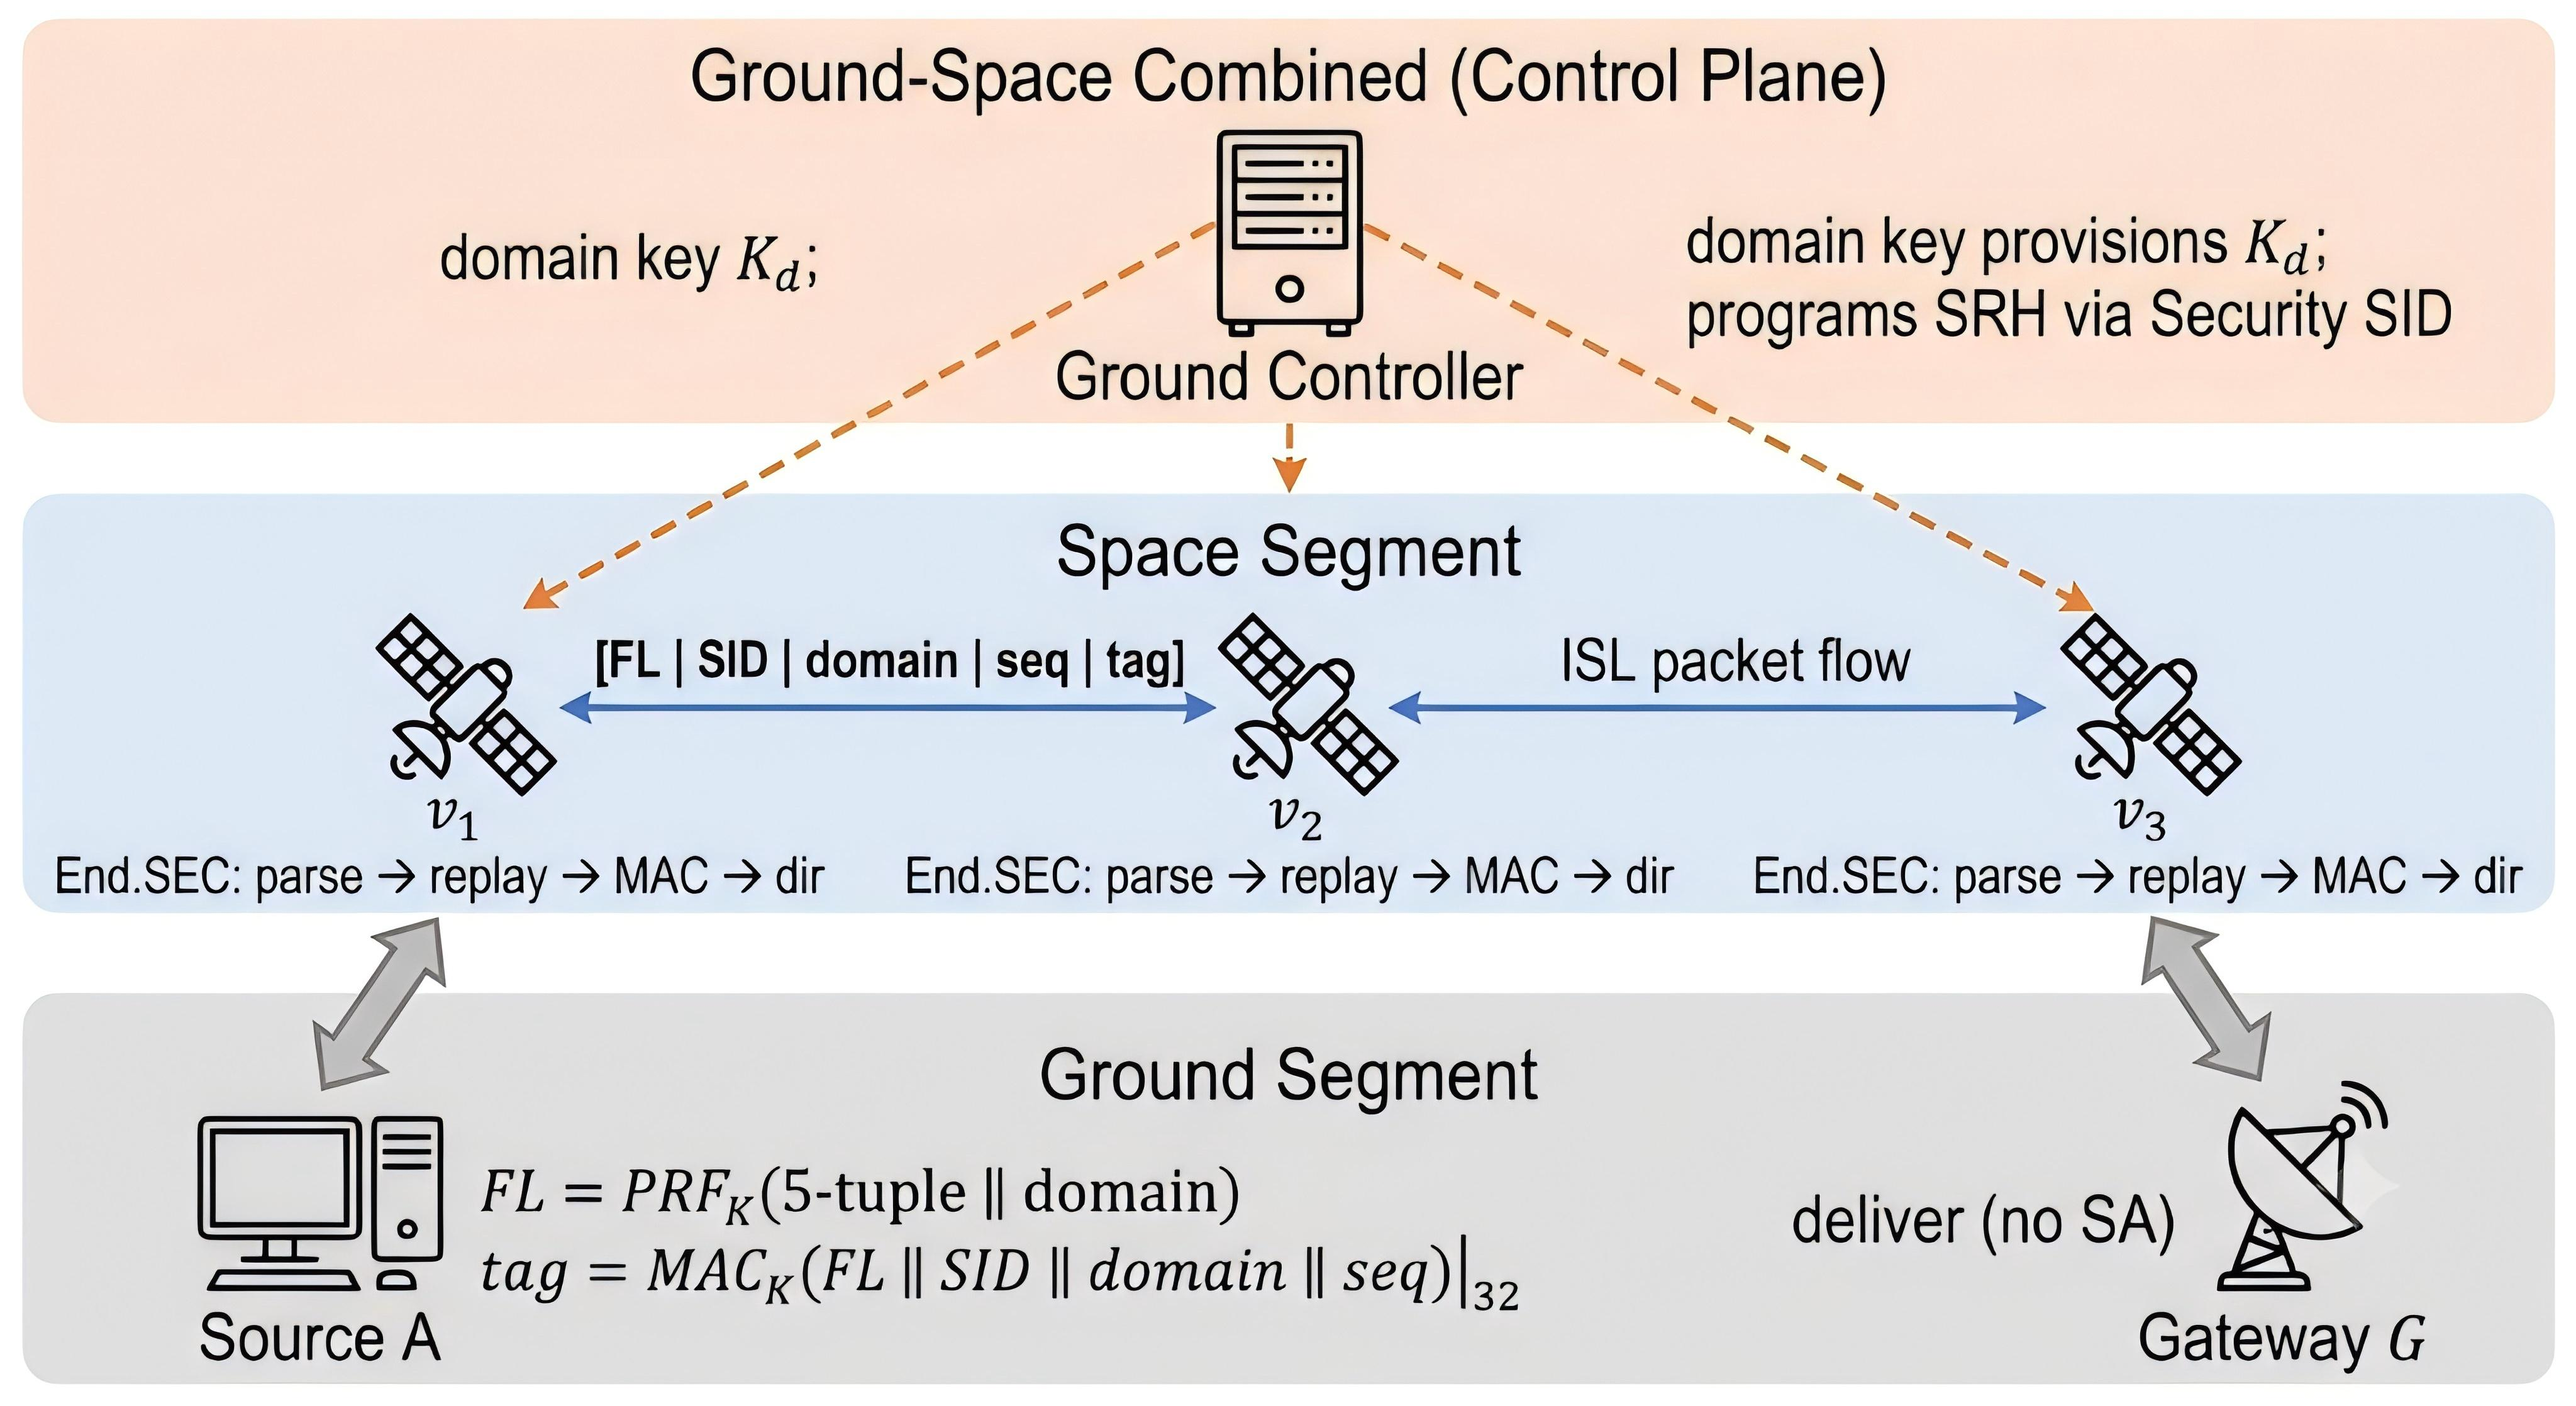
\includegraphics[width=\columnwidth]{figures/arch.jpg}
\caption{6FLAS three-segment architecture.}
\label{fig:arch}
\end{figure}

\subsection{Design Philosophy}
\label{sec:philosophy}

6FLAS carries security state in the packet rather than on
the satellite. Where stateful protocols store a security association per flow at
every protected node, 6FLAS derives a compact authenticator from a
domain key and embeds it in fields the packet already carries, so verifying
routers need no per-flow record. This drives the per-flow state term
$m_{\mathcal{M}}$ in \cref{eq:feasibility} toward zero and eliminates
ISL handover costs: when a flow is rerouted, no SA migrates because
none exists. The mechanism also exploits the structured LEO topology. Each
router forwards over a small fixed set of grid directions, so the egress access-control check
becomes a constant-time comparison
against the SID-encoded expected direction rather than a routing/policy lookup.

The immutable Flow Label supplies a stable, domain-authenticated flow-identity token
identical at every hop; the SRv6 Security SID supplies the per-hop path policy
and the bytes over which integrity is checked. \cref{fig:overview} shows the
resulting packet and the per-hop pipeline.

\begin{figure}[t]
\centering
\footnotesize
\setlength{\fboxsep}{4pt}
\fbox{\parbox{\dimexpr\columnwidth-2\fboxsep-2\fboxrule\relax}{\centering
\textbf{IPv6 base header} \;[\,\textbf{Flow Label} $\fl$ = $\prf_{\skey_\domid}(\text{5-tuple}\,\|\,\domid)$\,] \\[2pt]
$\downarrow$ \\[2pt]
\textbf{SRH} \;[\,Segment list $\;\dots\;$ \textbf{Security SID} = Loc$\,|\,$Func$\,|\,$Args\,] \\[2pt]
$\downarrow$ \\[2pt]
\textbf{6FLAS metadata (9\,B)}: \;[\,domain $\domid$ | seq $\seq$ | tag $\mtag$\,] \\[2pt]
$\downarrow$ \\[2pt]
\textbf{Payload} (optionally encrypted, out of scope)
}}
\caption{6FLAS packet structure.}
\label{fig:overview}
\end{figure}

\subsection{Flow-Label-Based Stream Authentication}
\label{sec:fl-auth}

\begin{definition}[Authenticated flow]
\label{def:flow}
A 6FLAS flow is the tuple $f=(\textsf{5tuple},\domid)$ where \textsf{5tuple} is
the IPv6 five-tuple (source/destination address, source/destination port,
next-header) and $\domid$ is a security-domain identifier shared by the
authorized routers serving the flow.
\end{definition}

The source node sets the Flow Label deterministically from the flow and the
domain key $\skey_\domid$:
\begin{equation}
\label{eq:fl}
\fl \;=\; \prf_{\skey_\domid}(\textsf{5tuple}\,\|\,\domid) \bmod 2^{20},
\end{equation}
where $\prf$ is a keyed pseudorandom function (using a SipHash-class keyed
PRF~\cite{siphash}). The label is then immutable in
transit~\cite{rfc6437}, serving as a stable, domain-authenticated flow identifier. Because $\skey_\domid$ is secret, an off-path adversary
cannot compute the label for a given five-tuple, and an on-path
adversary that copies $\fl$ cannot reuse it for a different authenticated routing context without detection (the per-packet MAC below binds them together). The 20-bit space
admits up to $2^{20}\approx 1.05$M concurrent labels per domain; collision
behavior under heavy load is discussed in the evaluation.

Each packet carries a 9-byte 6FLAS metadata block: a 1-byte domain id $\domid$,
a 4-byte sequence number $\seq$, and a 4-byte truncated MAC tag
\begin{equation}
\label{eq:tag}
\mtag \;=\; \mac_{\skey_\domid}\!\bigl(\textsf{IPv6.src} \,\|\, \textsf{IPv6.dst} \,\|\, \fl \,\|\, \textsf{SID} \,\|\, \domid \,\|\, \seq\bigr)\big|_{32},
\end{equation}
computed over the authenticated routing context: the IPv6 source and destination addresses (32\,B total, immutable in transit), the Flow Label (carried in the IPv6 header), the active Security SID (128 bits), the domain id, and the sequence number. Hop-variable fields such as Hop Limit and Segments Left are excluded to enable stateless per-hop verification. A verifying router recomputes the tag from
the packet fields plus the domain key it holds. No per-flow state is
consulted. The tag binds the routing endpoints and flow identity ($\textsf{IPv6.src/dst}$ and $\fl$), the active forwarding segment
(\textsf{SID}), and the freshness ($\seq$) together, so altering any of them
invalidates the tag (R1, R2). Note that 6FLAS authenticates routing context, not the full transport-layer five-tuple (which would require parsing layer-4 headers); this is consistent with its focus on hop-by-hop routing security rather than end-to-end transport-layer authentication. The 32-bit truncation's forgery probability is bounded in \cref{sec:security}.

The 4-byte sequence counter $\seq$ is a \emph{per-domain} counter: the source node (or a coordinated set of sources within a domain) maintains a single monotonically increasing counter for that domain, shared across all flows originating from it. This design allows the replay window to be indexed by $(\domid, \text{direction})$ rather than per flow, and the window check can operate directly on $\seq$ without tracking per-flow state. With 32 bits, the counter can represent over $4.2$ billion packets, providing ample headroom for typical domain traffic rates and multi-day key rotation intervals. At $10^4$\,pkt/s, a 32-bit counter wraps in approximately $5$ days, comfortably exceeding typical key rotation periods (hours to days). A 24-bit variant (3-byte $\seq$, 8-byte metadata) is feasible for low-rate domains or deployments with frequent key rotation (every 10--20 minutes), but 32 bits is the recommended baseline for general deployments.
Domain-key rotation implicitly resets the sequence space. The per-$(\domid, \text{direction})$ replay window $W_v[\domid, d]$ uses a
$w=256$-entry bitmap (32\,B per window). For a constellation serving $D$ domains over six $+$Grid directions, the total on-board state is
$D \times 6 \times 32$\,bytes, independent of the flow
count. For $D=256$ domains, this is $48$\,KB, small enough to reside in on-chip SRAM on representative space-grade processors.

\subsection{SRv6 Security Segment and Per-Hop Verification}
\label{sec:srv6-bind}

6FLAS encodes its per-hop policy in an SRv6 Security SID that follows the
standard \texttt{Locator$\,|\,$Function$\,|\,$Arguments} layout~\cite{rfc8986}.
The \texttt{End.SEC} function is defined as a strict superset of \texttt{End},
so nodes that implement only \texttt{End} continue forwarding without
interruption.

\begin{definition}[Security SID behavior \texttt{End.SEC}]
\label{def:endsec}
When a router $v$ receives a packet whose active SID carries the \texttt{End.SEC}
function code, it executes \cref{alg:verify} before performing the standard
SRv6 \texttt{End}/\texttt{End.X} forwarding action. If any check in
\cref{alg:verify} fails, the packet is dropped and no SRv6 processing occurs.
If all checks pass, $v$ advances the Segments Left pointer, applies the standard
SRv6 forwarding action for the next SID, and advances the replay window. Nodes
that implement \texttt{End} but not \texttt{End.SEC} perform standard
\texttt{End}/\texttt{End.X} forwarding without the security checks.
\end{definition}

\begin{itemize}
    \item \textbf{Locator} (64\,b): routes the packet toward the next 6FLAS node,
    exactly as in standard SRv6.
    \item \textbf{Function} (16\,b): a code point \texttt{End.SEC} that triggers
    6FLAS verification before the usual \texttt{End}/\texttt{End.X} forwarding.
    \item \textbf{Arguments} (48\,b): the path security policy, encoding the
    expected ingress direction, the authorized egress direction (one of the six
    fixed LEO grid directions), and a domain/policy tag matched against $\domid$.
\end{itemize}

Encoding the expected egress direction in the SID is what lets a router enforce
access control (R4) without a routing-table or policy lookup: the controller
that programs the path writes the intended next direction into the SID at
source time, and each hop simply checks that its actual forwarding direction
matches. \cref{tab:args} shows the 48-bit Arguments field layout.

\begin{table}[t]
\centering
\caption{6FLAS Security SID Arguments field (48 bits total).}
\label{tab:args}
\renewcommand{\arraystretch}{1.2}
\begin{tabular}{lrl}
\toprule
\textbf{Field} & \textbf{Bits} & \textbf{Description} \\
\midrule
Ingress dir.   & 4  & Expected ingress dir.\ (3\,b index + 1\,b reserved) \\
Egress dir.    & 4  & Authorized egress dir.\ (3\,b index + 1\,b reserved) \\
Domain id      & 8  & Matches $\domid$ in 6FLAS metadata block \\
Path-policy    & 32 & Controller-set policy hash for the flow group \\
\bottomrule
\end{tabular}
\end{table}

\paragraph{Per-hop verification}
\label{sec:perhop}
\cref{alg:verify} gives the per-hop procedure. After parsing the IPv6 base
header and the active SID, the router (1) uses the SID-encoded egress direction to index the per-direction replay-window table in $O(1)$,
(2) checks the sequence number against the sliding window for anti-replay (R3),
(3) recomputes the MAC of \cref{eq:tag} and compares it in constant time to the
carried tag (R1, R2), and (4) checks that the SID-encoded egress direction is
one of the node's authorized directions before forwarding (R4). Every step uses
only fields in the packet and the domain key; there is no per-flow SA lookup.

\begin{algorithm}[t]
\caption{6FLAS per-hop verification at router $v$}
\label{alg:verify}
\begin{algorithmic}[1]
\Require packet $p$; domain keys $\{\skey_\domid\}$; replay windows $W_v[\domid, d]$ indexed by domain and direction
\State $(\textsf{IPv6.src}, \textsf{IPv6.dst}, \fl,\textsf{SID},\domid,\seq,\mtag) \gets \textsc{Parse}(p)$
\If{$\domid \notin$ authorized domains at $v$} \State \textbf{drop} \EndIf
\State $\text{dir} \gets \textsc{EgressDir}(\textsf{SID.Args})$ \Comment{Extract egress direction from SID}
\State $w \gets W_v[\domid, \text{dir}]$ \Comment{$O(1)$ lookup by domain and direction}
\If{$\seq \le w.\text{base}$ \textbf{or} $w.\text{seen}(\seq)$}
    \State \textbf{drop} \Comment{Replayed or stale (R3)}
\EndIf
\State $\mtag' \gets \mac_{\skey_\domid}(\textsf{IPv6.src} \,\|\, \textsf{IPv6.dst} \,\|\, \fl \,\|\, \textsf{SID} \,\|\, \domid \,\|\, \seq)\big|_{32}$
\If{$\mtag' \neq \mtag$} \State \textbf{drop} \Comment{Forged or tampered (R1, R2)} \EndIf
\If{$\text{dir} \notin$ authorized directions at $v$}
    \State \textbf{drop} \Comment{Policy violation (R4)}
\EndIf
\State $w.\textsc{Advance}(\seq)$; \quad \textsc{ApplySRv6}(p); \quad \textbf{forward}
\end{algorithmic}
\end{algorithm}

A general router enforcing an egress policy would consult a forwarding or
policy table whose size grows with the number of destinations. In a $+$Grid LEO
node the authorized egress set has at most six members (north/south intra-plane,
east/west inter-plane, up/down ground), so line~13 of \cref{alg:verify} is a
comparison against a six-element fixed set, i.e., constant time and constant
space, independent of $|\setF|$. Likewise the replay window table $W_v[\domid, d]$ is sized
per $(\domid, \text{direction})$ pair, not per flow, so its memory is $O(D)$ in the number of domains rather than $O(|\setF|)$ in the flow count. These
specializations are what make 6FLAS satisfy the feasibility condition
\cref{eq:feasibility} at $10^6$ flows where stateful schemes do not. The only
mutable state a 6FLAS router keeps is the bounded per-$(\domid, \text{direction})$ replay window
$W_v[\domid, d]$, independent of the number of flows: many flows from the same domain going in the same direction share the same window,
and the window only tracks recently seen sequence numbers within the window lifetime (determined by the per-bucket arrival rate $R_{\domid,d}$ and the window size $w$).
Thus $m_{\mathcal{M}}$ per flow is effectively zero, and
a handover that reroutes a flow requires no state transfer, directly satisfying
D2 and D3.

\cref{alg:verify} decomposes into four stages with no inter-stage feedback:
(1)~header parse and domain-id gate, (2)~replay-window probe,
(3)~MAC recompute, and (4)~direction check and window advance.
Stages~2 and~4 access only the per-$(\domid, \text{direction})$ SRAM described above (48\,KB for 256 domains); stage~3
feeds the keyed-MAC core directly from parsed header fields with no memory
indirection. Because stage~3 is the critical-path stage (${\approx}264$\,ns at
1\,GHz), throughput is limited by the MAC core rather than any data-dependent
memory access, and a pipelined implementation sustains one verification per
MAC-core cycle. This four-stage, feed-forward pipeline maps directly onto an
FPGA or ASIC realization on a space-grade logic fabric~\cite{li2022}: the
critical path is a fixed-width keyed-hash, and the only state written back per
packet is a single bit in the per-$(\domid, \text{direction})$ replay bitmap.

\subsection{Domain Key Management}
\label{sec:keymgmt}

6FLAS verification requires each authorized router to hold the domain key
$\skey_\domid$. A full key-management protocol is out of scope~\cite{tan2025crossdomain},
but the stateless design keeps the overhead light. The domain key is a symmetric
secret shared among all nodes in domain $\domid$ --- including authorized ground
senders and verifying satellites. This means 6FLAS provides \emph{domain-origin}
authentication: a verifying router confirms the packet was minted by a node that
holds $\skey_\domid$, but cannot distinguish one authorized sender from another
within the same domain. Intra-domain source spoofing (one authorized sender
forging another's flow identifier) is outside the threat model; if per-sender
accountability within a domain is required, it must be layered above 6FLAS,
e.g.\ via an end-to-end signature over the payload.

The baseline 6FLAS design assumes each domain has a single authoritative packet source (or a coordinated set of sources that implement a distributed monotonic counter service). This is consistent with typical LEO ground-segment architectures where a domain corresponds to a managed ground gateway or a small set of co-located terminals under unified operational control. Multi-sender domains that cannot implement centralized sequence coordination have two options: (a) partition the 32-bit sequence space by sender ID (e.g., top 8 bits identify the sender, bottom 24 bits are the per-sender counter), or (b) revert to per-flow sequence numbering at the cost of increased on-board replay-window state (trading off the stateless advantage). The per-domain counter design reflects a deliberate trade: eliminating per-flow on-board state in exchange for domain-level sequence coordination, which is feasible in managed ground segments but may require additional infrastructure in fully decentralized deployments.

Each satellite is provisioned at manufacture or via
a secured telecommand channel with the keys of the domains it serves.
Ground terminals acting as packet sources are similarly provisioned through
the same ground-based key-management channel, since computing $\fl$ and the initial tag both require $\skey_\domid$.
The security perimeter of a domain thus spans all authorized senders and
verifiers sharing $\skey_\domid$.

Rotation follows an epoch schedule: the operator pushes $\skey_{\domid}^{(e+1)}$ to all
nodes before epoch $e{+}1$ begins. Verifiers accept both the current and the
immediately previous epoch to absorb in-flight packets. Because updates are
domain-granular, bandwidth scales as $O(|D|)$, not $O(|\setF|)$ --- for 256
domains with 128-bit keys, each epoch push is only $4096$\,bytes. Revocation
rotates the affected domain key and immediately invalidates any traffic an
adversary could mint. Because 6FLAS holds no per-flow secrets, revocation
granularity is the domain, which is coarse but cheap.

Consider a packet from source $A$ to gateway $G$
routed through on-board nodes $v_1{\to}v_2{\to}v_3$ in domain $\domid{=}7$.
Source $A$ computes $\fl=\prf_{\skey_7}(\textsf{5tuple}\,\|\,7)\bmod 2^{20}$,
sets $\seq$ from its per-domain counter (shared with all other sources in domain 7), and computes
$\mtag=\mac_{\skey_7}(\textsf{IPv6.src}\,\|\,\textsf{IPv6.dst}\,\|\,\fl\,\|\,\textsf{SID}\,\|\,7\,\|\,\seq)|_{32}$.
Each hop $v_i$ verifies the tag, checks $\seq$ against its per-$(\domid, \text{direction})$ replay window $W_v[7, d]$,
confirms the egress direction matches the SID-encoded policy, and forwards.
No node creates or consults a per-flow record. If an ISL break reroutes the flow through $v_2'$,
that node verifies the next packet with $\skey_7$ immediately, without re-keying.
